\documentclass[DIV16,BCOR1cm,10pt,a4paper,fleqn,twoside]{scrreprt}         % for pdf output
%\documentclass[DIV16,BCOR1cm,10pt,a4paper,fleqn]{scrreprt}         % for pdf output
%\documentclass[DIV16,BCOR1cm,11pt,a4paper,fleqn]{report}         % for pdf output

% To allow automatic selection of the right graphics type ...
% preset \pdfoutput for older latex installation, it is allways definted for
% news ones
\ifx\pdfoutput\undefined
\gdef\pdfoutput{0}
\fi

\newif\ifpdfx
\ifnum\pdfoutput=0
% latex is called for dvi output
   \pdfxfalse
   \usepackage{graphicx}
\else
% pdflatex is called for pdf output
   \pdfxtrue
   \usepackage[pdftex]{graphicx}
   \usepackage[pdftex]{hyperref}
\fi

\usepackage{textcomp}

%\newcommand{\CDO}{{\bfseries\sffamily CDO\ }}
\newcommand{\CDO}{{\bfseries\sffamily CDO}}
\newcommand{\cdologo}{
\includegraphics{logo/cdo_logo}}

\graphicspath{{figures/}}

% To define headers and footers
\usepackage{fancyhdr}
\pagestyle{fancy}

% Headers and footers personalization using the `fancyhdr' package
\fancyhf{} % Clear all fields

\renewcommand{\headrulewidth}{0.2mm}
\renewcommand{\footrulewidth}{0.2mm}

\renewcommand{\chaptermark}[1]{\markboth{#1}{}}
\renewcommand{\sectionmark}[1]{\markright{#1}}

%\renewcommand{\chaptermark}[1]{\markboth{#1}{}}
%\renewcommand{\sectionmark}[1]{\markleft{#1}}

\fancyhead[LO,RE]{\slshape \leftmark}
\fancyhead[LE,RO]{\slshape \rightmark}
\fancyfoot[LE,RO]{\Large\thepage}
%\fancyfoot[LO,RE]{\raisebox{-2.8mm}{\scalebox{0.17}{\cdologo}}}
\fancypagestyle{plain}{%
  \fancyhead{} % get rid of headers
  \renewcommand{\headrulewidth}{0pt}
}

%\setlength{\footnotesep}{0cm}
%\setlength{\footskip}{-2cm}
%\renewcommand{\footnoterule}{\rule{0cm}{0cm}}

\usepackage{exscale}
\usepackage{array,colortbl}    % color table

\usepackage{listings}
\usepackage{longtable}
\usepackage{color}
\definecolor{pcolor1}{rgb}{0.992, 0.980, 0.875}  % rgb: 253/250/223
\definecolor{pcolor2}{rgb}{1.000, 0.925, 0.700}  % rgb: 255/236/278
\definecolor{pcolor3}{rgb}{0.968, 0.756, 0.623}  % rgb: 247/193/159

%\usepackage{ae}               % fuer die "almost european" computer modern fonts
%\usepackage{url}              % Standard-Paket fuer WWW-Adressen

%\typearea{10}                 % Einen sinnvollen Satzspiegel aktivieren


%Usage:
%pdflatex cdo.tex
%pdflatex cdo.tex
%cat > cdo.ist << 'EOF'
%delim_0        "{\\idxdotfill} "
%headings_flag  1
%heading_prefix "{\\centerline {\\Large \\bf "
%heading_suffix "}}"
%EOF
%makeindex -s cdo.ist cdo.idx
%pdflatex cdo
%thumbpdf cdo
%pdflatex cdo


\usepackage{thumbpdf}

%\usepackage{html}

\usepackage{makeidx}

%\ifpdf
%\usepackage[a4paper, colorlinks=true, pdfstartview=FitV, bookmarks=true, linkcolor=blue,
%            citecolor=blue, urlcolor=blue, latex2html=true]{hyperref}
%\fi

\usepackage{hyperref}
\hypersetup{pdftoolbar=true,
            pdfmenubar=true,
            pdfwindowui=true,   
%            pdffitwindow=true,
            pdfauthor={Uwe Schulzweida},
            pdftitle={CDO Climate Data Operators},
            pdfcreator={pdflatex + hyperref},
            pdfstartview=FitV,
%            pdfpagemode=FullScreen,
            a4paper,
            bookmarks=true,
            linkcolor=blue,
            citecolor=blue,
            urlcolor=blue,
            colorlinks=true}

\setlength{\parindent}{0em}
\setlength{\parskip}{1.5ex plus0.5ex minus0.5ex}
\extrarowheight1pt

\makeindex
%\newcommand{\ii}[1]{\textit{#1}}  \newcommand{\nn}[1]{#1n}
%\renewcommand{\dotfill}{\leaders\hbox to 5p1{\hss.\hss}\hfill}
%\newcommand{\idxdotfill}{5p1{\hss.\hss}\hfill}
\newcommand{\idxdotfill}{\ \dotfill \ }
%\def\idxdotfill{\leaders\hbox to.6em{\hss .\hss}\hskip 0pt plus 1fill}
%\MakeShortVerb{\@}

\renewcommand{\indexname}{Operator index}

\newenvironment{defalist}[1]
{\begin{list}{}
{\settowidth{\labelwidth}{#1\ \ }
\setlength{\itemsep}{0mm}
\setlength{\itemindent}{0mm}
%\setlength{\listparindent}{25mm}
\setlength{\leftmargin}{\labelwidth}
%\setlength{\leftmargin}{25mm}
\setlength{\labelsep}{2mm}
\addtolength{\leftmargin}{\labelsep}
%\addtolength{\leftmargin}{8mm}
}}
{\end{list}}

\newenvironment{defalist2}[1]
{\begin{list}{}
{\settowidth{\labelwidth}{#1\ \ }
\setlength{\itemsep}{0mm}
\setlength{\itemindent}{0mm}
%\setlength{\listparindent}{25mm}
\setlength{\leftmargin}{\labelwidth}
%\setlength{\leftmargin}{25mm}
\setlength{\labelsep}{2mm}
\addtolength{\leftmargin}{\labelsep}
\addtolength{\leftmargin}{8mm}
}}
{\end{list}}

\newcommand{\miniwidth}{\textwidth}

\setcounter{secnumdepth}{3}

\begin{document}


\begin{titlepage}
\vspace*{50mm}
{\Huge{\bf CMOR support in \CDO}}

\setlength{\unitlength}{1cm}
\begin{picture}(16,0.4)
\linethickness{1.5mm}
%\put(0,0.1){\line(1,0){15.85}}
\put(0,0.1){\line(1,0){16.3}}
\end{picture}
\begin{flushright}
\large\bf{CMORizing of climate model data \\ October 2016}
\end{flushright}

\vfill

\Large{\bf Karl--Hermann Wieners, Uwe Schulzweida}

\Large{\sl Max Planck Institute for Meteorology}

\Large{\bf Mathis Rosenhauer}

\Large{\sl Deutsches Klimarechenzentrum (DKRZ)}

\begin{picture}(16,1)
\linethickness{1.0mm}
%\put(0,0.7){\line(1,0){15.85}}
\put(0,0.7){\line(1,0){16.3}}
\end{picture}
\end{titlepage}

\tableofcontents

\chapter{Introduction}

The Climate Data Operators ({\CDO}) software is a collection of operators
for standard processing of climate and forecast model data.

This document describes the additional {\CDO} operator cmor. This
operator is an interface to the CMOR library version 3 from PCMDI.
The CMOR support is available with {\CDO} release 1.8.0 or later.

The CMOR (Climate Model Output Rewriter) library comprises a set of
functions, that can be used to produce CF-compliant NetCDF files that 
fulfill the requirements of many of the climate community's standard
model experiments. These experiments are collectively referred to as
MIP's and include, for example, AMIP, CMIP, CFMIP, PMIP, APE, and IPCC 
scenario runs. The output resulting from CMOR is "self-describing" and
facilitates analysis of results across models.

Much of the metadata written to the output files is defined in
MIP-specific tables, typically made available from each MIP's web
site. CMOR relies on these tables to provide much of the metadata 
that is needed in the MIP context, thereby reducing the programming 
effort required of the individual MIP contributors.

The CDO operator cmor reads the data with the internal IO library CDI
and writes the NetCDF result directly with the CMOR library. 

\chapter{Building CDO with CMOR}

This section describes how to build and install {\CDO} with CMOR
support on a UNIX system.

\section{CMOR}
 
CMOR version 3 needs to be installed before building {\CDO}.
CMOR depends on the following external libraries:
netCDF-4.0 , HDF5, UDUNITS-2, zlib and uuid.
Make sure that you use exactly the same libraries for the {\CDO}
installation, otherwise the operator cmor will possibly not working correctly.

\section{Compilation}

First go to the {\CDO}  \href{https://code.zmaw.de/projects/cdo}{\tt download} page
({\tt https://code.zmaw.de/projects/cdo}) to get the latest distribution,
if you do not have it yet.
Compilation is done by performing the following steps:

\begin{enumerate}
\item Unpack the archive, if you haven't done that yet:
   
\begin{verbatim}
    gunzip cdo-$VERSION.tar.gz    # uncompress the archive
    tar xf cdo-$VERSION.tar       # unpack it
    cd cdo-$VERSION
\end{verbatim}

\item Configure {\CDO} with CMOR support:

The configuration depends on the location of the external libraries. Here is one example:

\begin{verbatim}
./configure --with-cmor=<CMOR root directory> --with-netcdf=<NetCDFroot directory> \
            --with-uuid --with-udunits2 LIBS=-lossp-uuid                           \
            CPPFLAGS="-I<CMOR root dir>/include/cdTime -I<CMOR root dir>/include/json-c"
\end{verbatim}

For an overview of other configuration options use

\begin{verbatim}
    ./configure --help
\end{verbatim}

\item Compile the program by running make:

\begin{verbatim}
    make
\end{verbatim}

\end{enumerate}

The program should compile without problems and the binary ({\tt cdo}) 
should be available in the {\tt src} directory of the distribution.


\section{Installation}

After the compilation of the source code do a {\tt make install},
possibly as root if the destination permissions require that.

\begin{verbatim}
    make install
\end{verbatim} 

The binary is installed into the directory {\tt $<$prefix$>$/bin}.
{\tt $<$prefix$>$} defaults to {\tt /usr/local} but can be changed with 
the {\tt --prefix} option of the configure script. 


\chapter{\label{refman}CMOR operator reference manual}

This section gives a description of all {\CDO} operators to generate plots.
Related operators are grouped to modules.
For easier description all single input files are named \texttt{ifile} or \texttt{ifile1}, \texttt{ifile2}, etc.,
and an arbitrary number of input files are named \texttt{ifiles}.
All output files are named \texttt{ofile} or \texttt{ofile1}, \texttt{ofile2}, etc.


\hspace{3mm}

\input{ref_list_cmor}
\input{ref_man_cmor}


\begin{thebibliography}{xx}


\bibitem[CDI]{CDI} \ \\
  \href{https://code.zmaw.de/projects/cdi}
       {Climate Data Interface},
  from the
  \href{http://www.mpimet.mpg.de}
       {Max Planck Institute for Meteorologie}


\bibitem[CDO]{CDO} \ \\
  \href{https://code.zmaw.de/projects/cdo}
       {Climate Data Operators},
  from the
  \href{http://www.mpimet.mpg.de}
       {Max Planck Institute for Meteorologie}


\bibitem[CMOR]{CMOR} \ \\
  \href{git://github.com/PCMDI/cmor.git}
       {Climate Model Output Rewriter},
  from the
  \href{https://www-pcmdi.llnl.gov}
       { Program For Climate Model Diagnosis and Intercomparison (PCMDI)}


\end{thebibliography}


%\appendix

% \chapter{\label{appendixpingo}Hints for PINGO user}
% 
% Some {\CDO} operators have the same name as in PINGO but
% the meaning is different.
% The following table gives an overview of those operators.
% 
% \vspace{2mm}
% \begin{tabular}[c]{|l||l|l|}
% \hline
% Operator name  & {\CDO}                   & PINGO \\
% \hline
% \hline
% min            & Minimum of two fields  & Time minimum \\
% \hline
% max            & Maximum of two fields  & Time maximum \\
% \hline
% daymean        & Daily mean             & Multi-year daily mean \\
% \hline
% daymin         & Daily minimum          & Multi-year daily minimum \\
% \hline
% daymax         & Daily maximum          & Multi-year daily maximum \\
% \hline
% monmean        & Monthly mean           & Multi-year monthly mean \\
% \hline
% monmin         & Monthly minimum        & Multi-year monthly minimum \\
% \hline
% monmax         & Monthly maximum        & Multi-year monthly maximum \\
% \hline
% seasmean       & Seasonally mean        & Multi-year seasonally mean \\
% \hline
% \end{tabular}
% \vspace{2mm}
% 
% There are also some {\CDO} operators with the same functionality
% as in PINGO but the name is different.
% The following table gives an overview of those operators.
% 
% \vspace{2mm}
% \begin{tabular}[c]{|l||l|l|}
% \hline
%                              & {\CDO}       & PINGO \\
% \hline
% \hline
% Maximum of two fields        & max        & max2 \\
% \hline
% Minimum of two fields        & min        & min2 \\
% \hline
% Field mean, min, max         & fldmean, fldmin, fldmax    & meanr minr, maxr\\
% \hline
% Time mean, min, max          & timmean, timmin, timmax    & mean, min, max \\
% \hline
% Daily mean, min, max         & daymean, daymin, daymax    & daymeans, daymins, daymaxs \\
% \hline
% Monthly mean, min, max       & monmean, monmin, monmax    & monmeans, monmins, monmaxs \\
% \hline
% Yearly mean, min, max        & yearmean, yearmin, yearmax   & yearmeans, yearmins, yearmaxs \\
% \hline
% Running mean                 & runmean    & runmeans \\
% \hline
% Seasonally mean              & seasmean   & seasmeans \\
% \hline
% Multi-year daily mean        & ydaymean   & daymean  \\
% \hline
% Multi-year monthly mean      & ymonmean   & monmean  \\
% \hline
% Multi-year seasonally mean   & yseasmean  & seasmean  \\
% \hline
% \end{tabular}
% \vspace{2mm}



\chapter{\label{appendixgrid}Grid description examples}

\section{Example of a curvilinear grid description}
Here is an example for the {\CDO} description of a curvilinear grid.
xvals/yvals describes the position of the 6x5 quadrilateral grid cells.
The first 4 values of xbounds/ybounds are the corners of the first grid cell.
\lstset{moredelim=**[is][\color{red}]{|}{|}}
\begin{lstlisting}[frame=single, backgroundcolor=\color{pyellow}, basicstyle=\footnotesize]
gridtype  = curvilinear
gridsize  = 30
xsize     = 6
ysize     = 5
xvals     =  |-21|  -11    0   11   21   30  -25  -13    0   13
              25   36  -31  -16    0   16   31   43  -38  -21
               0   21   38   52  -51  -30    0   30   51   64
xbounds   =  |-23  -14  -17  -28|       -14   -5   -6  -17        -5    5    6   -6
               5   14   17    6        14   23   28   17        23   32   38   28
             -28  -17  -21  -34       -17   -6   -7  -21        -6    6    7   -7
               6   17   21    7        17   28   34   21        28   38   44   34
             -34  -21  -27  -41       -21   -7   -9  -27        -7    7    9   -9
               7   21   27    9        21   34   41   27        34   44   52   41
             -41  -27  -35  -51       -27   -9  -13  -35        -9    9   13  -13
               9   27   35   13        27   41   51   35        41   52   63   51
             -51  -35  -51  -67       -35  -13  -21  -51       -13   13   21  -21
              13   35   51   21        35   51   67   51        51   63   77   67
yvals     =   |29|   32   32   32   29   26   39   42   42   42
              39   35   48   51   52   51   48   43   57   61
              62   61   57   51   65   70   72   70   65   58
ybounds   =   |23   26   36   32|        26   27   37   36        27   27   37   37
              27   26   36   37        26   23   32   36        23   19   28   32
              32   36   45   41        36   37   47   45        37   37   47   47
              37   36   45   47        36   32   41   45        32   28   36   41
              41   45   55   50        45   47   57   55        47   47   57   57
              47   45   55   57        45   41   50   55        41   36   44   50
              50   55   64   58        55   57   67   64        57   57   67   67
              57   55   64   67        55   50   58   64        50   44   51   58
              58   64   72   64        64   67   77   72        67   67   77   77
              67   64   72   77        64   58   64   72        58   51   56   64
\end{lstlisting}

\begin{figure}[b]
\ifpdfoutput{
{\scalebox{0.99}{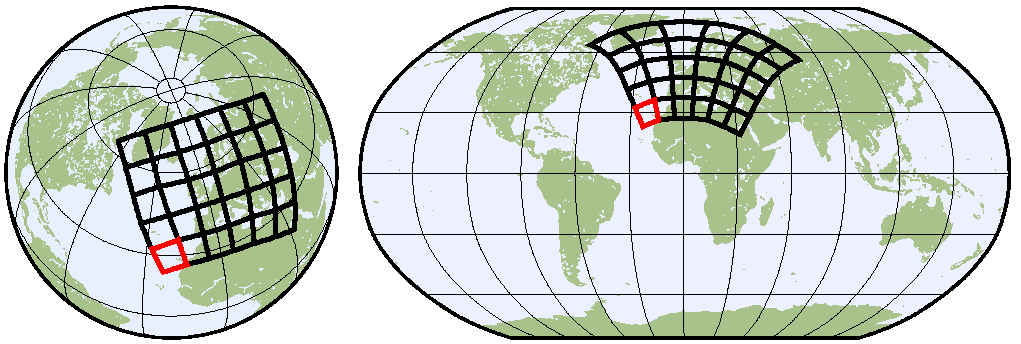
\includegraphics{grids/curv.pdf}}}
}{
{\scalebox{0.99}{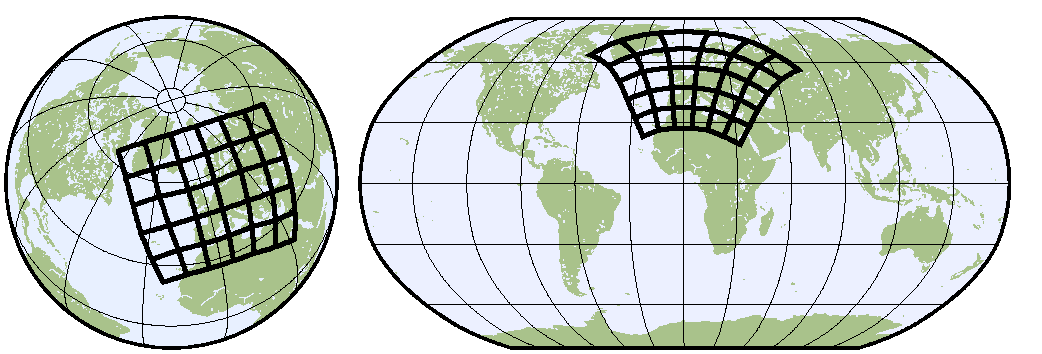
\includegraphics{grids/curv}}}
}
\caption[curvgrid]{Orthographic and Robinson projection of the
  curvilinear grid,  the first grid cell is colored red}
\end{figure}

\newpage
\section{Example description for an unstructured grid}
Here is an example of the {\CDO} description for an unstructured grid.
xvals/yvals describes the position of 30 independent hexagonal grid cells.
The first 6 values of xbounds/ybounds are the corners of the first
grid cell. The first grid cell is colored red.
\begin{lstlisting}[frame=single, backgroundcolor=\color{pyellow}, basicstyle=\footnotesize]
gridtype  = unstructured
gridsize  = 30
nvertex   = 6
xvals     =  |-36|   36    0  -18   18  108   72   54   90  180  144  126  162 -108 -144 
            -162 -126  -72  -90  -54    0   72   36  144  108 -144  180  -72 -108  -36 
xbounds   =  |339    0    0  288  288  309|        21   51   72   72    0    0
               0   16   21    0  339  344       340    0   -0  344  324  324
              20   36   36   16    0    0        93  123  144  144   72   72
              72   88   93   72   51   56        52   72   72   56   36   36
              92  108  108   88   72   72       165  195  216  216  144  144
             144  160  165  144  123  128       124  144  144  128  108  108
             164  180  180  160  144  144       237  267  288  288  216  216
             216  232  237  216  195  200       196  216  216  200  180  180
             236  252  252  232  216  216       288  304  309  288  267  272
             268  288  288  272  252  252       308  324  324  304  288  288
             345  324  324   36   36   15        36   36  108  108   87   57
              20   15   36   57   52   36       108  108  180  180  159  129
              92   87  108  129  124  108       180  180  252  252  231  201
             164  159  180  201  196  180       252  252  324  324  303  273
             236  231  252  273  268  252       308  303  324  345  340  324
yvals     =   |58|   58   32    0    0   58   32    0    0   58   32    0    0   58   32 
               0    0   32    0    0  -58  -58  -32  -58  -32  -58  -32  -58  -32  -32 
ybounds   =   |41   53   71   71   53   41|        41   41   53   71   71   53
              11   19   41   53   41   19       -19   -7   11   19    7  -11
             -19  -11    7   19   11   -7        41   41   53   71   71   53
              11   19   41   53   41   19       -19   -7   11   19    7  -11
             -19  -11    7   19   11   -7        41   41   53   71   71   53
              11   19   41   53   41   19       -19   -7   11   19    7  -11
             -19  -11    7   19   11   -7        41   41   53   71   71   53
              11   19   41   53   41   19       -19   -7   11   19    7  -11
             -19  -11    7   19   11   -7        11   19   41   53   41   19
             -19   -7   11   19    7  -11       -19  -11    7   19   11   -7
             -41  -53  -71  -71  -53  -41       -53  -71  -71  -53  -41  -41
             -19  -41  -53  -41  -19  -11       -53  -71  -71  -53  -41  -41
             -19  -41  -53  -41  -19  -11       -53  -71  -71  -53  -41  -41
             -19  -41  -53  -41  -19  -11       -53  -71  -71  -53  -41  -41
             -19  -41  -53  -41  -19  -11       -19  -41  -53  -41  -19  -11
\end{lstlisting}

\begin{figure}[b]

\ifpdfoutput{
{\scalebox{1}{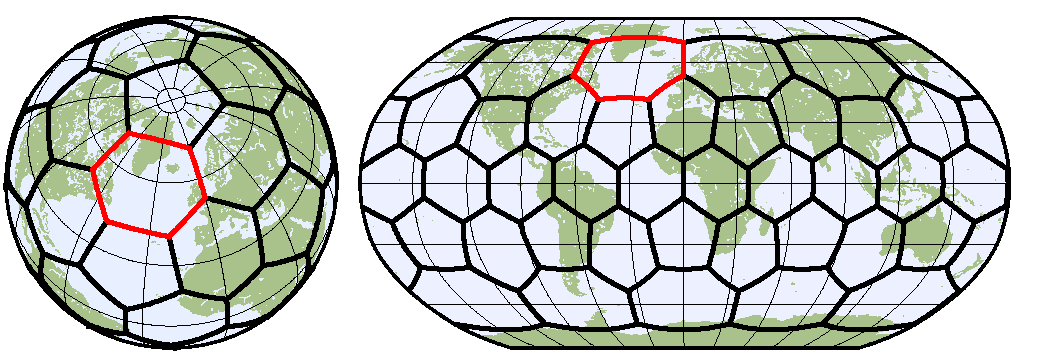
\includegraphics{grids/cell.pdf}}}
}{
{\scalebox{1}{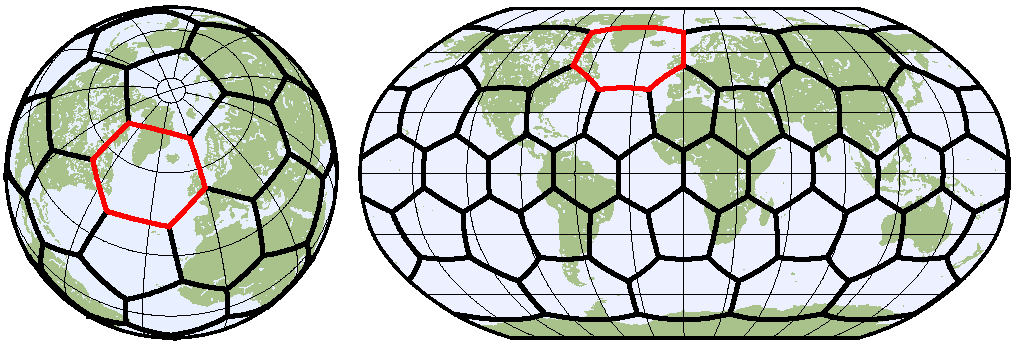
\includegraphics{grids/cell}}}
}
\caption[cellgrid]{Orthographic and Robinson projection of the unstructured grid}
\end{figure}

%%% Local Variables: 
%%% mode: latex
%%% TeX-master: "grid"
%%% End: 


\clearpage
\ifpdfx
\phantomsection
\addcontentsline{toc}{chapter}{\indexname}
\printindex
\else
\input{catalog}
\input{alphabetic_list}
\fi
\end{document}
